\documentclass{article}

% if you need to pass options to natbib, use, e.g.:
% \PassOptionsToPackage{numbers, compress}{natbib}
% before loading nips_2017
%
% to avoid loading the natbib package, add option nonatbib:
% \usepackage[nonatbib]{nips_2017}

\PassOptionsToPackage{numbers, compress}{natbib}
\usepackage{nips_2017}

% to compile a camera-ready version, add the [final] option, e.g.:
% \usepackage[final]{nips_2017}

\usepackage[utf8]{inputenc} % allow utf-8 input
\usepackage[T1]{fontenc}    % use 8-bit T1 fonts
\usepackage{hyperref}       % hyperlinks
\usepackage{url}            % simple URL typesetting
\usepackage{booktabs}       % professional-quality tables
\usepackage{amsfonts}       % blackboard math symbols
\usepackage{nicefrac}       % compact symbols for 1/2, etc.
\usepackage{microtype}      % microtypography

%for matrices
\usepackage{blkarray}
\usepackage{amsmath}

\usepackage{graphicx}
\usepackage{caption}
\usepackage{subcaption}

\usepackage[svgnames, table]{xcolor} % Enabling colors by their 'svgnames'

% define custom commands
\definecolor{commentPJA_color}{rgb}{1.0,0.0,0.8}
\newcommand{\commentPJA}[1]{{\textcolor{commentPJA_color}{PJA: #1}}}


% define custom commands
\definecolor{commentLP_color}{rgb}{1.0,0.0,0.8}
\newcommand{\commentLP}[1]{{\textcolor{commentLP_color}{LP: #1}}}


% define custom commands
\definecolor{commentAP_color}{rgb}{1.0,0.0,0.8}
\newcommand{\commentAP}[1]{{\textcolor{commentAP_color}{AP: #1}}}

% define custom commands
\definecolor{commentRJ_color}{rgb}{1.0,0.0,0.8}
\newcommand{\commentRJ}[1]{{\textcolor{commentRJ_color}{RJ: #1}}}


\newcommand{\mb}[1]{\mathbf{#1}}
\newcommand{\bs}[1]{\boldsymbol{#1}}
\newcommand{\mvec}[1]{\mathbf{#1}}

\title{Givens Transform Approach for Efficient Probabilistic Principle Component Analysis for Bayesian Dimensionality Reduction (GT-PPCA)}

% The \author macro works with any number of authors. There are two
% commands used to separate the names and addresses of multiple
% authors: \And and \AND.
%
% Using \And between authors leaves it to LaTeX to determine where to
% break the lines. Using \AND forces a line break at that point. So,
% if LaTeX puts 3 of 4 authors names on the first line, and the last
% on the second line, try using \AND instead of \And before the third
% author name.

\author{
  David S.~Hippocampus\thanks{Use footnote for providing further
    information about author (webpage, alternative
    address)---\emph{not} for acknowledging funding agencies.} \\
  Department of Computer Science\\
  Cranberry-Lemon University\\
  Pittsburgh, PA 15213 \\
  \texttt{hippo@cs.cranberry-lemon.edu} \\
  %% examples of more authors
  %% \And
  %% Coauthor \\
  %% Affiliation \\
  %% Address \\
  %% \texttt{email} \\
  %% \AND
  %% Coauthor \\
  %% Affiliation \\
  %% Address \\
  %% \texttt{email} \\
  %% \And
  %% Coauthor \\
  %% Affiliation \\
  %% Address \\
  %% \texttt{email} \\
  %% \And
  %% Coauthor \\
  %% Affiliation \\
  %% Address \\
  %% \texttt{email} \\
}

\begin{document}
% \nipsfinalcopy is no longer used

\maketitle

\begin{abstract}
We develop scalable and flexible Probabilistic Principal Component Analysis (PPCA) methods for determining posterior distributions of spanning frames based on a Givens Representation of the PCA which we term (GT-PPCA).  This addresses significant challenges that arise with latent variable in a traditional formulation of PPCA.  For sampling posterior distributions we develop Hamiltonian Monte-Carlo Methods (HMC) for sampling on the Stiefel Manifold the PCA orthogonal frame sets.  We demonstrate our approach on several challenging example problems including tests problems XYZ and problems arising in  our recent work on understanding medical patient data associated with coagulopathy (factors influencing blood clotting).  We show our methods provides ways to identify when data sets contain a mixture of low dimensional structures that would not be resolved with traditional PCA approaches.  We further show how our approach can be used to develop heirarchical models in terms of low dimensional structures learned from the data sets or to develop prior distributions useful in generalizing low dimensional structures to new settings.  To facilitate use of our GT-PPCA method we provide a package with the widely-used Stan statistics package.  
\end{abstract}

%%%%%%%%%%%%%%%%%%%%%%%%%
\section{Introduction}
%%%%%%%%%%%%%%%%%%%%%%%%%

%\commentPJA{For later, Try to bring forth the novelty of our methods earlier in introduction while explaining the traditional PCA.  Best to have first draft and then streamline at the end after all materials together.}

Principal Component Analysis (PCA) is a widely used dimensionality-reduction tool for exploratory analysis and modeling in both the natural and social sciences. By factorizing an empirical covariance matrix into a product of low rank matrices, PCA effectively finds a low dimensional subspace that describes the dataset in terms of the latent factors.  These factors are given by the columns of the low rank factorization.  Geometrically, traditional PCA can be interpreted as providing a point estimate of a low dimensional hyper-plane that is closest to a cloud of data points.  For binary or integer valued matrices, such as graph adjacency matrices arising in network science, Matrix Factorization (NMF) \citep{lee2001algorithms} or Exponential Family PCA (EPCA) \citep{collins2001generalization} are often used to find such low dimensional latent factors.

Probabilistic PCA (PPCA) \citep{tipping1999probabilistic} and Bayesian Exponential Family PCA (BXPCA) \citep{mohamed2009bayesian}, posit probabilistic generative models that are equivalent to PCA in the limit of decreasing noise \citep[chapt.~12.2]{murphy2012machine}. This probabilistic approach is attractive because it allows a straightforward way, via Bayesian inference, to quantify the uncertainty in our estimates (to prevent overfitting) and conduct hypothesis testing. For example, given high-dimensional fMRI scans of a human brain under two different settings, it would be desirable to find a posterior distribution of low-dimensional subspaces that describe the data, then find the probability given the data that these subspaces, or latent factors are different under the two settings. While uncertainty quantification of the latent factors in PPCA has been explored in the literature \citep{hoff2009simulation,brubaker2012family, byrne2013geodesic}, there are currently no out-of-the-box solutions available to researchers. 

In addition to allowing uncertainty quantification and hypothesis testing, probabilistic models are amenable to expansion and can serve as modules within larger probabilistic graphical models. This is important in real-world settings where true generative models are often complex and where they do not necessarily follow the simple generative process set forth by PPCA. Following the fMRI example, a situation could arise where we believe brain scans from people of different age groups may be described by different low-dimensional representations, but that the respective representations for each group all come from some hierarchical prior distribution. In such a case it would be desirable to build a hierarchical model \cite[chapt.~5]{gelman2014bayesian} of latent factors, but such expanded PPCA models have not been explored much, let alone implemented as a package for general use by researchers and scientists.

\paragraph{Bayesian inference of orthonormal matrices} Many of the difficulties in conducting full Bayesian inference on PPCA and related models stem from having to infer one or more unknown orthonormal matrices.  This is difficult because orthonormal matrices form a rather particular subset of all possible realizable matrices; this yields a probability measure on a sub-manifold within the full space of matrices with a non-trivial geometry.  More specifically, the prior and posterior distributions of an orthonormal matrix $W$ must have support over the set of $n \times p$ orthonormal matrices.  This is known as the Stiefel manifold and denoted $V_{n,p}$ \citep{muirhead2009aspects}.  When first considering this problem, it may seem that this geometry may rule out a straight-forward use of two of the most prominent techniques for posterior inference posterior inference, Markov Chain Monte Carlo (MCMC) and Variational Inference (VI).  Intuitively, for MCMC, we have no way of guaranteeing that a chain over $W$ will explore only valid regions of parameter space that satisfy the orthonormality constraints. Similarly for Variational Inference, positing a common variational posterior distribution such as a Gaussian over the elements of $W$ are sure to lead to posteriors that assign mass to invalid regions of parameter space.

In the case of positively constrained parameters, posterior distributions are in practice rather routinely inferred using both MCMC and VI. This can be accomplished by transforming the constrained variables to an unconstrained space using the one-to-one mapping $f: \mathrm{supp}(z_\mathrm{constr}) \to \mathbb{R}^D$, where $\mathrm{supp}(z_\mathrm{constr})$ is the support of the constrained random variable $z_\mathrm{constr}$ \citep{carpenter2016stan, kucukelbir2014fully}. To our knowledge, no such transformation has been proposed to map orthonormal matrices to a comparable unconstrained space.

\paragraph{GT-PPCA} In this paper we draw on techniques from Differential Geometry and Numerical Analysis to introduce a novel and geometrically elegant way to represent orthonormal matrices.  In our approach  we express orthonormal matrices in terms of a sequence of fundamental rotations through given angles. This gives insight in to the geometry of the Stiefel manifold, and results in a transform we call the Givens Transform, that maps orthonormal matrices to an unconstrained space. We apply the Givens Transform to inference of PPCA-based models, and collectively refer to this as GT-PPCA.

GT-PPCA is straight-forward to implement in stand-alone inference schemes, but is particularly useful in the context of a probabilistic programming languages like Stan \citep{carpenter2016stan}, where we can use it for uncertainty quantification and hypothesis testing of PPCA models, as well as extending PPCA to more complex probabilistic graphical models, two previously difficult tasks. We provide Stan code for our example models allowing for use by researchers and scientists out-of-the-box, and we show how inference of these models in Stan yields good empirical performance in diverse applications such as hierarchical subspace modeling for fMRI data and sparse PPCA for medical data.

Furthermore, GT-PPCA gives insight in to novel and useful ways to work with and interpret our models.  For instance, the elegant geometric representation lets us see how by limiting the range of the parameters in GT-PPCA, we can naturally avoid naturally avoid issues of unidentifiability and multi-modal posteriors that arise in other methods.  GT-PPCA also allows us new and creative ways to generate and use prior distributions on orthonormal matrices.  In the setting of using the matrix directly this task has previously been rather complicated and rather intractable for even small problem sizes.  This is linked to the difficulty of evaluating densities of orthonormal matrix distributions in other representations.  As we shall discuss in more detail, our GT representation provides a rather natural way to specify prior distributions comparable to the Matrix Langevin prior \citep{muirhead2009aspects}.

\paragraph{Related work} To address these issues, there has been some recent work on posterior inference of orthonormal matrices based on modified versions of Hamiltonian Monte Carlo (HMC) with sampling for constrained parameters (cite).  These methods use modified numerical integrators to ensure that exploration only occurs in valid areas of parameter space where the necessary constraints are satisfied (cite).  Because these methods use modified integrators for constrained parameters, they require approaches in practice for keeping track of the type of each variable and for which type of integrator to use on each variable. This adds an extra layer of algorithmic complexity, especially for large complex probabilistic graphical models.  This further makes it difficult to implement these methods in a scalable fashion and within widely used probabilistic programming languages and packages, such as Stan \citep{carpenter2016stan}. Furthermore, we have found while these methods represent some progress on this challenging problems the numerical methods are sometimes not rigorous or robust and at times can suffer from errors and instabilities that jeopardize the integrity of samples.  In addition, we have found these methods can at times induce unnecessary multi-modality that are an artifact of the chosen respresentation and not intrinsic to the model under study.  This arises in part from the choice of representations directly in terms of unconstrained matrices in these methods (cite).  As a consequence, the matrix in the PPCA model has equal liklihood when making an arbitrary change of sign of one of its columns.  Given this equivalent relation this can result in significant multi-modality that must be handled with some care in the final analysis.

\paragraph{Paper outline} We give a brief overview of probabilistic dimensionality reduction in Section~\ref{Probabilistic dimensionality reduction}.  We discuss how orthonormal matrices arise naturally for performing inference and introduce a precise description of the Stiefel manifold in Section~\ref{orthonormal}.  We also briefly review prior work on 
Bayesian dimensionality reduction using orthonormal matrices in Section~\ref{orthonormal}.  We introduce the Givens Transform (GT) and use for reductions to obtain our representations in Section~\ref{Givens}.  We also discuss practical consideration for GT in computing and using the representation in Section~\ref{Givens}.  We then show how our methods can be used in practice for Bayesian inference on a few probabilistic graphical models in Section (ref).  This includes illustration of the basic aspexcts of the technique on XYZ and presenting a more advanced real-world application to patient data for factors affecting coagulapathy in Section (ref).  We conclude discussing how our GT-PPCA methods can be utilized on other problems and by discussing our implimentation in Stan that can be utlized by others interested in our approach.

%%%%%%%%%%%%%%%%%%%%%%%%%


%%%%%%%%%%%%%%%%%%%%%%%%%
\section{Probabilistic Dimensionality Reduction} \label{Probabilistic dimensionality reduction}
%%%%%%%%%%%%%%%%%%%%%%%%%

\commentPJA{Discuss general context here... linear dimensinoality reductions... motivations briefly etc...}

\commentPJA{Discuss specific approach... PPCA...}

\subsection{Probabilistic Principle Component Analysis (PPCA)}
In probabilistic principle component analysis (PPCA) one starts by considering a collection of data points in a typically high-dimensional vector space and seeks to find a posterior distribution over a reduced representations of the data using a much lower dimensional subspace.  The central postulate is that for a data vector $\mathbf{x} \in \mathbb{R}^n$ there exists an unknown low-dimensional latent representation $\mathbf{z} \in \mathbb{R}^p$ where $p < n$, (ideally with $p \ll n$).  The two representations are related to each other by a single unknown linear transformation $\mathbf{x} \rightarrow \mathbf{z}$.  Mathematically, we consider a finite collection of sampled data vectors $\mathbf{x}^i \in \mathbb{R}^n$, $i = 1, \cdots, N$ and see and estimate of the subspace.  Formally, in PPCA this consists of using the following generative process
\begin{eqnarray}
\label{eq:PpcaGenerativeProcess}
p(\mb{z}^i) &\sim& \mathcal{N}_p(0, I) \nonumber\\
p(\mb{x}^i | \mb{z}^i, W, \Lambda, \sigma^2) &\sim& \mathcal{N}_n(W \Lambda \mb{z}^i, \sigma^2 I).
\end{eqnarray}
The $W$ is an $n \times p$ orthonormal matrix and $\Lambda$ is a $p \times p$ diagonal matrix with positive elements.  For simplicity in our presentation of PPCA, we have assumed here that the data has only zero mean but the more general case can also readily be considered (cite).
%PJA: Avoid footnotes...\footnote{we assume the zero mean case here for simplicity, but the more general case easily follows}. 
We also remark that generative model could also be expanded to the case of non-Gaussian data by replacing equation \ref{eq:PpcaGenerativeProcess} with an exponential family member whose natural parameters are given by $\mathrm{Expon}(W\Lambda \mb{z}^i)$ where $\mathrm{Expon}(\cdot)$ is an appropriate link function \citep{mohamed2009bayesian}. 

%%%%%%%%%%%%%%%%%%%%%%%%%
%\subsection{Bayesian inference of orthonormal matrices}
%%%%%%%%%%%%%%%%%%%%%%%%%

\subsection{Importance of the Orthonormality Condition}
\label{orthonormal}
We mention that the orthonormal constraint on the matrix $W$ plays an important role in obtaining robust methods for
in making inferences in probabilistic PCA.  If one were to relax the orthonomal constraint the likelihood function would assign identical probability to a whole equivalence class of matrices $W \sim V$ where the span is the same linear subspace $\mbox{span}\{W\} = \mbox{span}\{V\}$.  While this might not seem theoretically too problematic, in practice this presents a number of major challenges.  This first is that the matrices in a given equivalence class are not all equally well-conditioned numerically in defining the linear subspace and round-off errors and truncation errors become problematic in practical calculations .  Secondly, these issues with the representation further manifest in the log-likihood objective function where regions arise of particularly large curvature.  This causes significant numerical issues for variational inference (VI) in nonlinear optimization methods and in monte-carlo (MC) approaches with samplers having slow mixing times~
\citet[chapt.~12.1.3]{murphy2012machine, mohamed2009bayesian,holbrook2016bayesian}.  These issues render making inferences in PPCA with such non-orthonormal matrices impractical resulting from a statistics stand-point in effective unidentifiability.

\subsection{Inference using the Stiefel Manifold}
To develop robust approaches for PPCA we restrict inferences to be over matrices that are constrained to be orthonormal~\citet[chapt.~12.1.3]{murphy2012machine}.  In the space of $n\times p$ orthonormal matrices defines the Stiefel Manifold~\citep{muirhead2009aspects}
\begin{equation}
V_{n,p} := \{Y \in \mathbb{R}^{n \times p}: YY^T = I \}.
\end{equation}
The Stiefel Manifold has an intrinsic dimension of $\dim{V^{n,p}} = np-p(p+1)/2$.  This airses from the constraints on the columns of the matrix that impose orthonormality.  This dimensionality can be seen by observing, that the first column of $Y \in V_{n,p}$ must have norm one and hence has one constraint placed on it. The second column must also have norm one and also must be orthogonal to the first column hence with two constraints placed on it.  Continuing to the third column through the $n^{th}$ one arrives at the conclusion that each point of the Stiefel Manifold has only $np-p(p+1)/2$ degrees of freedom.  We shall discuss how to develop coordinate-charts for  representing points within the Stiefel Manifold using Givens transformations in Section (ref).


%%%%%%%%%%%%%%%%%%%%%%%%%
\subsection{Givens Transform (GT) approach to PPCA (GT-PPCA)} \label{Givens}
%%%%%%%%%%%%%%%%%%%%%%%%%

\commentPJA{I would give a streamlined discussion of the GT-PPCA approach giving the basics of the GT and how the representation is used.}


\commentPJA{I will move much of the material below to an appendix for now and move pieces or re-writes up into this section as needed to make clear.  Can always refer reader t the Appendix for the more technical parts.  A streamlined discussion GT should be given enough to develop the PPCA, but not too much technicalities on differential geometry and all the rest that an expert could piece together.  It is an art at what level to cover things and I can certaintly help with that.  }



\begin{figure}
    \centering
    \begin{subfigure}[b]{0.3\textwidth}
        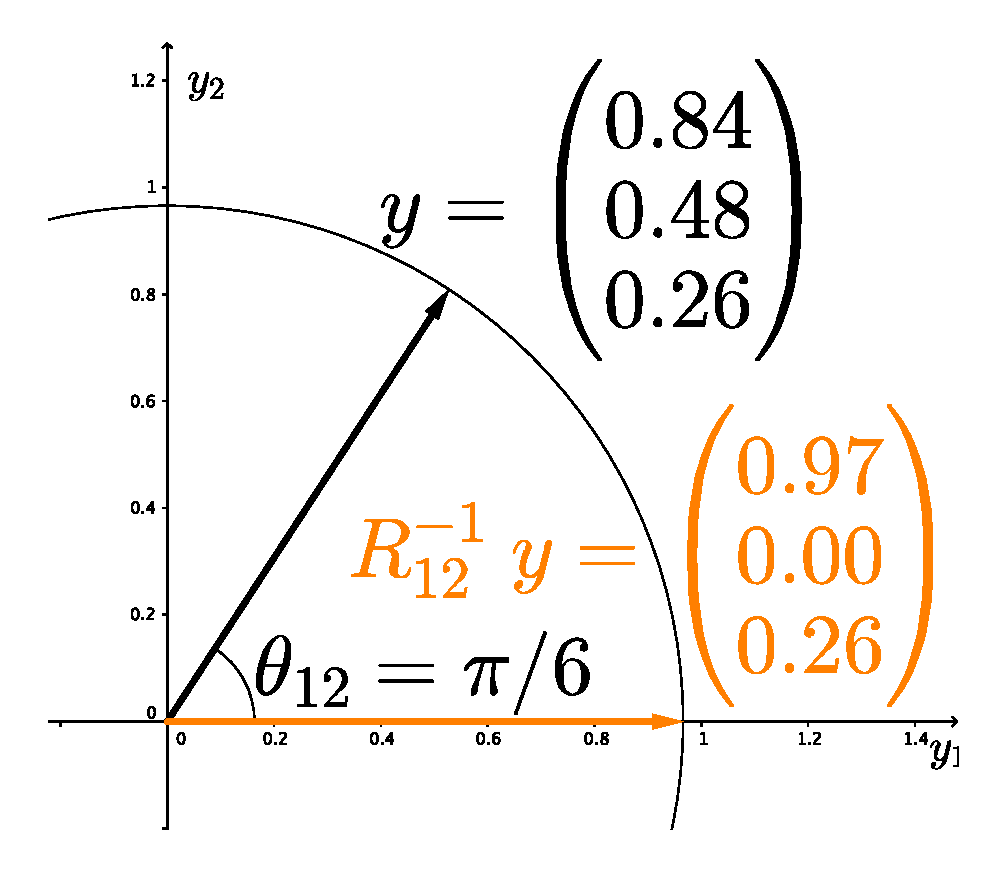
\includegraphics[width=\textwidth]{GivensReduction.pdf}
        \caption{}
        \label{fig:GivensReduction}
    \end{subfigure}
    ~ %add desired spacing between images, e. g. ~, \quad, \qquad, \hfill etc. 
      %(or a blank line to force the subfigure onto a new line)
    \begin{subfigure}[b]{0.3\textwidth}
        \includegraphics[width=\textwidth]{StiefelGeom.pdf}
        \caption{}
        \label{fig:StiefelGeom}
    \end{subfigure}
    ~ %add desired spacing between images, e. g. ~, \quad, \qquad, \hfill etc. 
    %(or a blank line to force the subfigure onto a new line)
    \begin{subfigure}[b]{0.3\textwidth}
        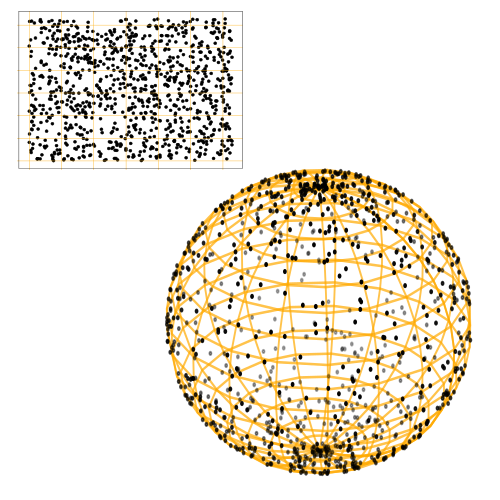
\includegraphics[width=\textwidth]{AreaForm.pdf}
        \caption{}
        \label{fig:AreaForm}
    \end{subfigure}
    \caption{Visualizing the Givens Transform. (a) How the Givens Reduction ``zeros out'' a column vector. (b) A geometric view of the Stiefel manifold, two-frame in three dimensions. (c) Sampling without a proper measure adjustment. \commentPJA{Good start on figures.  Please remember to use vector format .PDF final output.  Can use Inkscape or Adobe Illustrator to process PDF and SVG files from plotters like Python Matplotlib or Matlab or Stan, etc... Please be sure to save both .SVGZ (source file) and .PDF files in Git repo. This allows for easy edits later to figures as needed.}  \commentPJA{Fonts are a little too small on Fig. a.  Color in Fig. b would be better to use light blue or something more neutral.   Use Red for labels... rember color balance.  Point sizes a little bigger in in-set in Fig. C.  Save both sphere dots and square separately and use Inkspace / Illustrator to combine.}  }\label{fig:Givens}
\end{figure}




%%%%%%%%%%%%%%%%%%%%%%%%%
\section{Examples}
%%%%%%%%%%%%%%%%%%%%%%%%%

%%%%%%%%%%%%%%%%%%%%%%%%%
\subsection{Synthetic Data}
Show how point estimation of subspace and dimensionality can be misleading. Show multi-modality of Symone's method.

%%%%%%%%%%%%%%%%%%%%%%%%%
\subsection{FMRI}
Illustrate hypothesis testing.

%%%%%%%%%%%%%%%%%%%%%%%%%
\subsection{School Network}
Mainly here to show we can do exponential families easy too. Possibly make this a change point detection?

%%%%%%%%%%%%%%%%%%%%%%%%%
\subsection{Coagulopathy using hierarchical subspace models}
Don't forget to mention sparse PCA, via Cauchy priors.

%%%%%%%%%%%%%%%%%%%%%%%%%
\section{Discussion}
%%%%%%%%%%%%%%%%%%%%%%%%%

\subsubsection*{Acknowledgments}

Use unnumbered third level headings for the acknowledgments. All
acknowledgments go at the end of the paper. Do not include
acknowledgments in the anonymized submission, only in the final paper.

%%%%%%%%%%%%%%%%%%%%%%%%%
%%%%%%%%%%%%%%%%%%%%%%%%%
%%%%%%%%%%%%%%%%%%%%%%%%%
\bibliographystyle{plainnat} % or try abbrvnat or unsrtnat
\bibliography{paperDatabase} % refers to example.bib

%%%%%%%%%%%%%%%%%%%%%%%%%
\section*{Appendix}
%%%%%%%%%%%%%%%%%%%%%%%%%


\subsection{Givens Reductions of Matrices}

\commentPJA{Give a basic description of the background on Givens reductions of a matrix that we can refer to with additional details than we need in the main text.}


\subsection{Differential Geometry of the Steifel Manifold}

\commentPJA{Discuss the basic differential geometry of the Steifel Manifold and how we handle these various issues.  Degenerate regions and metric factors (Jacobians).  Discuss how we use "multi-coordinate charts" when necessary to avoid being close to regions with bad metric factors and degeneracy, etc...}


\subsection{Reduction Matrices}

\[
R_{ij} := 
\begin{blockarray}{cccccccccccc}
 & & & i &  & & & j & & \\
\begin{block}{(ccccccccccc)c}
  1 &  &  &  &  & & & &  & & &  \\
   & \ddots &  &  & & & & &  & & &  \\
   &  & 1  &  &  & & & &  & & & \\
   & & & \cos \theta_{ij} &  & &  & -\sin \theta_{ij} &  & & & i \\
   & & & & 1  & &  & &  & & & \\
   & & &  & & \ddots  &  & &  & & &  \\
   & & &  & & & 1 & &  & & &  \\
   & & & \sin \theta_{ij}  &  & &  & \cos \theta_{ij} &  & & & j \\
   & & &  &  & &  & & 1 & & & \\
   & & &  &  & &  & & & \ddots & & \\
      & & &  &  & &  & & & & 1 & \\
\end{block}
\end{blockarray}
 \]

\begin{equation}
R_{12}^{-1} Y 
=
R_{12}^{-1}
\begin{pmatrix}
y_{11} & y_{12} & \cdots & y_{1p}\\
y_{21} & y_{22} & \cdots & y_{2p}\\
y_{31} & y_{32} & \cdots & y_{3p}\\
\vdots & \vdots & \vdots & \vdots\\
y_{p1} & y_{p2} & \cdots & y_{pp}\\
y_{p+1,1} & y_{p+1,2} & \cdots & y_{p+1,p}\\
\vdots & \vdots & \vdots & \vdots\\
y_{n1} & y_{n2} & \cdots & y_{np}\\
\end{pmatrix}
=
\begin{pmatrix}
* & * & \cdots & *\\
0 & * & \cdots & *\\
y_{31} & y_{32} & \cdots & y_{3p}\\
\vdots & \vdots & \vdots & \vdots\\
y_{p1} & y_{p2} & \cdots & y_{pp}\\
y_{p+1,1} & y_{p+1,2} & \cdots & y_{p+1,p}\\
\vdots & \vdots & \vdots & \vdots\\
y_{n1} & y_{n2} & \cdots & y_{np}\\
\end{pmatrix}.
\end{equation}

\begin{equation}
(R_{1n}^{-1} \cdots R_{13}^{-1} R_{12}^{-1}) Y 
=
\begin{pmatrix}
1 & 0 & \cdots & 0\\
0 & * & \cdots & *\\
0 & * & \cdots & *\\
\vdots & \vdots & \vdots & \vdots\\
0 & * & \cdots & *\\
0 & * & \cdots & *\\
\vdots & \vdots & \vdots & \vdots\\
0 & * & \cdots & *\\
\end{pmatrix}.
\end{equation}

\begin{equation}
(R_{2n}^{-1} \cdots R_{23}^{-1})
(R_{1n}^{-1} \cdots R_{12}^{-1}) Y 
=
\begin{pmatrix}
1 & 0 & \cdots & 0\\
0 & 1 & \cdots & *\\
0 & 0 & \cdots & *\\
\vdots & \vdots & \vdots & \vdots\\
0 & 0 & \cdots & *\\
0 & 0 & \cdots & *\\
\vdots & \vdots & \vdots & \vdots\\
0 & 0 & \cdots & *\\
\end{pmatrix}.
\end{equation}

Continuing in this fashion yields

\begin{equation}
(R_{pn}^{-1} \cdots R_{p,p+1}^{-1})
\cdots
(R_{2n}^{-1} \cdots R_{23}^{-1})
(R_{1n}^{-1} \cdots R_{12}^{-1}) Y 
=
\begin{pmatrix}
1 & 0 & 0 & 0\\
0 & 1 & 0 & 0\\
0 & 0 & \ddots & 0\\
0 & 0 & 0 & 1\\
\vdots & \vdots & \vdots & \vdots\\
0 & 0 & \cdots & 0\\
0 & 0 & \cdots & 0\\
\vdots & \vdots & \vdots & \vdots\\
0 & 0 & \cdots & 0\\
\end{pmatrix}
=
I_{np}.
\end{equation}

\section{Misc LaTeX}

\subsection{Related works using HMC}
\commentPJA{I'd move this material in some form to the introduction and give a brief overview of how out methods are different.  Then maybe mention briefly during discussions prior work when our approach differs and explain why (as you do below, but in a sentence or two in the particular context).}

Before discussing details of our approach in more detail, we briefly discuss related prior works.  Recently, two approaches to posterior inference of orthonormal matrices and other constrained parameters have been proposed. These methods work by modifying the leap-frog integrator used to simulate Hamiltonian dynamics in HMC to ensure that any trajectory in parameter space remains on the Stiefel manifold. \citet{brubaker2012family} uses the SHAKE integrator \citep{leimkuhler2004simulating} to ensure trajectories through parameter space continuously satisfy the required constraints. The integrator works by repeatedly taking a step forward that may be off the manifold using ordinary leap frog, then projecting back down to the nearest point on the manifold. This projection is done via Newton iterations, which may not converge in practice, possibly jeopardizing the ergodicity of a Markov chain.

\citet{byrne2013geodesic} took a different approach, exploiting the fact that closed form solutions are known for the geodesic equations over the Stiefel manifold in the embedded coordinates, $W$. While this method is completely explicit, requiring no Newton iterations, in practice we found that for larger step sizes, the integrator steps off the Stiefel manifold, due to the numerical imprecision of the matrix exponential function.

Both methods rely on applying different integrators to constrained parameters. This adds implementation difficulty in practice, as one must keep track of the type of each variable (unconstrained or constrained, and type of constraint), and apply the appropriate integrator. Additionally, we note that even using orthonormal matrices, the PPCA likelihood is equivalent for a matrix $W$ and any permutation of the columns of $W$ being negative. As such, these methods lead to multi-modal posteriors, that can be avoided in a straight-forward way, as we show in the next section, using the Givens transform.

%%%%%%%%%%%%%%%%%%%%%%%%%
\subsection{Givens Reductions}
%%%%%%%%%%%%%%%%%%%%%%%%%

\commentPJA{I've temporarily moved this to the misc text section, to be added back into the main exposition in a more streamlined way.}
We provide a brief exposition on Givens Reductions, which motivate the Givens Transform, then describe the Givens Transform along with relevant practical considerations.

Define $R_{ij}$ to be the $n \times n$ rotation matrix that performs a counter-clockwise rotation in the $(i,j)$-plane of $\mathbb{R}^n$, where $j > i$. In $\mathbb{R}^3$, there are three such matrices, $R_{12}$, $R_{13}$, and $R_{23}$. They perform counter-clockwise rotation of angle $\theta_{ij}$ in the $(x,y)$, $(x,z)$ and $(y,z)$ planes respectively. Rotation matrices have the following key properties:

\begin{enumerate}
\item They preserve length and angles between vectors, i.e. for two vectors $u,v \in \mathbb{R}^n$, $R_{ij} u, R_{ij} v$ are the same length as $u$ and $v$ respectively, and if $u$ and $v$ are orthogonal then so are $R_{ij}u$ and $R_{ij}v$.
\item They are invertible and their inverse is their transpose $R_{ij}^{-1} = R_{ij}^T$. Their inverse corresponds to a clockwise rotation in the $(i,j)$-plane.
\end{enumerate}

%%%%%%%%%%%%%%%%%%%%%%%%%
Now we consider an $n \times p$ matrix $Y$, with orthonormal columns. In general, the first column is a vector in $\mathbb{R}^n$ with a non-zero second element. However, we can apply an invertible clockwise rotation in the $(1,2)$-plane, $R_{12}^{-1}$, to ``zero out" the second element of the first column. Figure \ref{fig:GivensReduction} depicts this visually for a 3D vector projected on to the $(1,2)$-plane.


Similarly, we can apply consecutive rotations $R_{13}^{-1}, R_{14}^{-1}, \cdots, R_{1n}^{-1}$ to this result so that all entries of the first column besides the first element are zero. The first column of the resulting matrix, $R_{1n}^{-1} \cdots R_{13}^{-1}  R_{12}^{-1}Y$, will be the length one vector $(1 \, 0 \, \cdots \, 0)^T$ which lies entirely along the first axis. If one takes the perspective that these rotations are applied to the columns of $Y$, then with the two properties of rotation matrices we mentioned earlier, it is evident that columns 2 through $n$ must have zero in their first element because they will be orthogonal to the first column, $(1 \, 0 \, \cdots \, 0)^T$.

To ``zero out" the elements of the second column, one can similarly apply rotations $R_{23}^{-1}, \cdots, R_{2n}^{-1}$. These rotations will leave the first column and first row unaffected, as the first column no lies entirely on the 1st axis, which these rotations do not involve. Continuing in this fashion yields

\begin{equation}
\label{eq:GivensReduction}
(R_{pn}^{-1} \cdots R_{p,p+2}^{-1} R_{p,p+1}^{-1}) \cdots (R_{2n}^{-1} \cdots R_{24}^{-1} R_{23}^{-1})(R_{1n}^{-1} \cdots R_{13}^{-1}  R_{12}^{-1})Y = I_{n,p},
\end{equation}

where $I_{n,p}$ consists of the first $p$ columns of the $n \times n$ identity matrix. This process of applying consecutive rotation matrices to a matrix is known in numerical analysis as the Givens reduction \citep{meyer2000matrix}, and is applied more generally to square matrices for matrix-vector solves. In total we will have applied $(n-1)+(n-2)+\cdots+(n-p) = np -p(p+1)/2$ rotations matrices. We note that because rotation matrices are very sparse in high dimensions, multiplication by a rotation matrix is computationally much less intensive than matrix multiplication otherwise would be.

%%%%%%%%%%%%%%%%%%%%%%%%%%%%%
\subsection{Givens Transform}
Because rotation matrices are invertible, equation \ref{eq:GivensReduction} implies that we can rewrite the $n \times p$ orthonormal matrix $Y$ as the product of counter-clockwise rotation matrices and $I_{n,p}$:

\begin{equation}
\label{eq:GivensRepresentation}
Y = (R_{12} \cdots R_{1n}) \cdots (R_{23} \cdots R_{2n}) (R_{p+1,n} \cdots R_{pn}) I_{n,p}.
\end{equation}

Recall that each of the $np -p(p+1)/2$ rotation matrices have an associated  angle $(\theta_{12} \cdots \theta_{1n}) \cdots (\theta_{23} \cdots \theta_{2n}) (\theta_{p+1,n} \cdots \theta_{pn})$, that we collectively refer to as $\Theta$. In this way we have reparameterized all $n \times p$ orthonormal matrices \footnote{other than a set of measure zero we explain in the next subsection}, a constrained space, in terms of unconstrained angles \footnote{the angles are themselves constrained to lie in certain intervals e.g. $[0, \pi)$ but these sorts of constraints are routine to deal with using a one-to-one diffeomorphism between intervals and the real line e.g. the sigmoid transform}, using a transform $\Theta: V_{n,p} \to \mathbb{R}^{np -p(p+1)/2}$. We refer to \ref{eq:GivensRepresentation} as the Givens representation or Givens transform.

%%%%%%%%%%%%%%%%%%%%%%%%%%%%%
\subsubsection{A geometric perspective}
The Givens transform can be visualized in the simple case when $n = 3$ and $p = 2$. This is the case where data is three-dimensional and we seek a two-dimensional subspace to represent the data. In this case, we can imagine a two dimensional bases, visualized as two perpendicular vectors that rotate rigidly together along three angles of rotations. This is referred to as a 2-frame in differential geometry \citep{muirhead2009aspects} and is depicted in Figure \ref{fig:StiefelGeom}. Recall $\theta_{12}$ controls the amount of rotation in the $(1,2)$-plane, $\theta_{13}$ in the$(1,3)$-plane, and $\theta_{23}$ controls a rotation of the second basis vector about the first. All rotations will preserve the length and orthogonality of the basis vectors. Given a flat, pancake-like cloud of points in 3D, the two dimensional bases will move according to the appropriate angles to be aligned with the cloud of points, if one were conducting a (Maximum A-Posteriori) MAP estimation over the Stiefel manifold.

%%%%%%%%%%%%%%%%%%%%%%%%%%%%%
\subsubsection{Practical considerations of topology and angles}
Topologically, $V_{n,p}$ is locally equivalent to Euclidean space, but not globally equivalent, meaning it is impossible to find a one-to-one map between the Stiefel manifold and Euclidean space. Technically speaking, the Givens transform can map angles to all of $V_{n,p}$ except for a subset $S \subset V_{n,p}$, that in the $n=3, p=2$ case corresponds to a sliver when $\theta_{12} \in (-\pi, \pi)$, $\theta_{13} \in (-\pi/2, \pi/2)$, and $\theta_{23} \in (-\pi/2, \pi/2)$. Luckily this set is of measure zero (under the proper measure for the Stiefel manifold, see section \ref{differentialFormsSection}), and thus, with probability one, the orthonormal matrix that describes the true subspace our data lie in will not be in that set. 

In practice, we actually limit the angle $\theta_{12}$ to an interval of length $\pi$ rather than an integral of length $2\pi$, that traverses the entire Stiefel manifold. Examining the angles of the Givens transform makes it evident that in the latter case, two equivalent bases that are the negation of each other can be reached, resulting in a multi-modal posterior that makes sampling and VI more difficult and harder to interpret. To avoid this multi-modality using the modified integrator methods would require a mechanism to avoid boundaries, which are not as intuitively defined in the default embedded coordinates as in the Givens transform.

Lastly, we note that if the true bases lies near a pole, i.e. $\theta_{ij}$ is close to $-\pi/2$ or $\pi/2$, then posteriors will tend to be multi-modal as the region in parameter space close to the boundaries will be close to equally valid, while the region near zero, will not be valid and thus contain little probability mass. In these cases, one can simply change the chart so that $\theta_{ij} \in (0, \pi)$, creating a uni-modal posterior in the new coordinate system, and alleviating numerical issues. In Stan this is straight-forward, as one simply has to change the lower and upper bound of the angle parameter.

%%%%%%%%%%%%%%%%%%%%%%%%%%%%%
\subsubsection{Jacobian under a change of variables}
The Givens transform \ref{eq:GivensRepresentation} allows us to represent orthonormal matrices as angles $Y(\Theta)$. This in turn allows us to write probability densities $p_Y(Y)$ in terms of angles, so that we can conduct inference in an unconstrained space. It is well known in probability theory that the transform of a random variable is in general not the density of the transform, i.e. $p_\Theta(\Theta) \neq p_Y(Y(\Theta))$\citep[chapt.~2.6]{murphy2012machine}. To be more precise, densities are measured against volumes and integrated to get actual probabilities (otherwise known as probability mass). Under a transformation, densities are unaffected, but volumes (or rather the way in which volumes are measured) may change. This is important in the context of posterior inference, as not including the Jacobian adjustment would result in different priors than we intend.

Figure \ref{fig:AreaForm} depicts how samples that are uniform in the angle space are not uniform on the sphere. Samples congregate at the poles of the sphere because a patch of area in the angle space that is near the top corresponds to a very tiny patch of the sphere near the pole. In practice this would lead to posteriors that bias towards the poles, when what we really intend is a prior that is uniform on the Stiefel manifold.

For a $K$-dimensional random vector $Y$ and a transformation $f: \mathrm{supp}(Y) \to \mathbb{R}^K$ the proper way to measure probability under a transform is by multiplying by the determinant of the Jacobian of the the inverse transform:

\begin{equation}
\int p_\Theta(\Theta)\, d\Theta = \int p_Y(Y(\Theta)) |\det J_{f^{-1}}(\Theta)|\, d\Theta.
\end{equation}

In our case this poses a problem however, because an $n \times p$ orthonormal matrix is $np$-dimensional, but the Givens transform, $\Theta(Y)$, maps this set to a $np - p(p+1)2$-dimensional set. In this more general scenario, one can not simply take the determinant of the Jacobian as the volume morphing factor, because the Jacobian is not even square and hence the determinant is undefined. To obtain the correct factor one must appeal to the calculus of differential forms. 

%%%%%%%%%%%%%%%%%%%%%%%%%%%%%
\subsubsection{Differential forms}\label{differentialFormsSection}

We offer an intuitive high-level overview of differential forms. For a thorough account we recommend \citet{muirhead2009aspects}, \citet{edelman200518}, or any standard text in differential geometry. The simplest non-trivial example of differential-forms between spaces of different sizes arises when trying to measure probablity using spherical coordinates. Spherical coordinates give us a map from $\mathbb{R}^2$ to the sphere, $(\theta, \varphi) \mapsto (x(\theta,\varphi), y(\theta,\varphi), z(\theta,\varphi))$. Although a sphere lies in 3-D space, if we have a density $p_\mathrm{Euc}(x,y,z)$ on the sphere, the ``natural'' way to measure the probability of a spherical random variable falling within some area on the surface of that sphere is by first covering that area with tiny rectangles tangent to the sphere, taking the average density of each rectangle, multiplying that density by the area of that rectangle, and summing over the resulting products. The probability of the random variable falling within that area is defined to be the limit of that result as the size of the rectangles go to zero. Area forms, or two-forms can be thought of as these infitessimal rectangles. They are written as the wedge product of two differentials, e.g. $dx \wedge dy$, and they are objects that are inserted into integrals to obtain measures. Differential forms form (no pun intended) a vector space useful for measuring areas and high-dimensional volumes. For example, the area forms on a sphere can be written as a linear combination of the standard-basis two forms

\begin{equation}
\label{eq:EuclideanAreaForm}
a(x,y,z)\, dx \wedge dy + b(x,y,z)\, dx \wedge dz + c(x,y,z)\, dy \wedge dz.
\end{equation}

One can then integrate this over a sub-area of the sphere to obtain the measure of that sub-area. The beauty of differential forms is that a different coordinate system such as polar coordinates, simply correspond to using a different basis for representing forms, which again are vectors. In fact writing a form in a different bases simply involves taking partial derivatives, e.g. $dx = (\partial x/\partial \theta) \, d\theta + (\partial x/ \partial \varphi) \, d\varphi$. If we substitute the forms in the angle bases in to \ref{eq:EuclideanAreaForm} and simplify using the well-defined anti-symmetric and distributive properties of wedge products and differential forms (see \citep{muirhead2009aspects}), we obtain a proper area-form \ref{eq:EuclideanAreaForm} in spherical coordinates, $S(x(\theta, \varphi),y(\theta, \varphi),z(\theta, \varphi))\, d\theta \wedge d\varphi$, that can then be integrated using a double integral in polar coordinates. The absolute value of this area-form evaluated at some point specified in angle coordinates, $(\theta_0, \varphi_0)$, intuitively measures how much the area of tiny square in angle space gets shrunk or stretched when the area is mapped to an area on the sphere.

Analogously, we can measure volumes on the Stiefel manifold. For $n \times p$ orthonormal matrices, there are only $np-p(p+1)/2$ free parameters and so the proper form to measure sets of orthonormal matrices is in fact a $np-p(p+1)/2$-form. For an orthonormal, $n \times p$ matrix, $Y$, we can find an orthonormal $n \times n$ matrix $G$ such that $G^T Y = I_{n,p}$. In fact $G$ just comes from the product of the appropriate rotation matrices that comes from the Givens Reduction \ref{eq:GivensReduction}. \citet{muirhead2009aspects} shows that the correct form comes from wedging the elements of the $n \times p$ matrix $G^T dY$ that lie below the diagonal i.e.

\begin{equation}
\label{eq:WedgeForm}
\bigwedge_{i=1}^p \bigwedge_{j=i+1}^n G_j^T\, dY_i
\end{equation}

where $G_j$ is the $j$th column of $G$ and $Y_i$ is the $i$th column of $Y$. To obtain the form in angle coordinates we simply obtain $dY$ in angle coordinates. $dY_i$ can be obtained in terms of the angle coordinates by the following relationship, $dY_i = J_{Y_i}(\Theta)\, d\Theta$, where $J_{Y_i}$ is the Jacobian of $Y_i$ with respect to the angle coordinates. Once we obtain the form \ref{eq:WedgeForm} in terms of the angle coordinates, the result is a wedge product of $np-p(p+1)/2$ vectors that are $np-p(p+1)/2$ dimensional, which reduces to the determinant of these vectors aligned side by side as a $np-p(p+1)/2 \times np-p(p+1)/2$ matrix. This determinant is analogous to and serves the same purpose as Jacobian adjustment that comes from transforming random variables. We can insert it in to the log-probability of a model to avoid the sort of unintended sampling behavior depicted in Figure \ref{fig:AreaForm}. We incorporate the form \ref{eq:WedgeForm} in to the log-probability of all of our Stan examples.



\end{document}
